\chapter{Experimental Setup}
\label{chap:experimental_setup}

In the following, we will outline the experimental setup for the experiments we ran.
This includes not only allocation, preprocessing and pair selection of each dataset, but also a description and motivation for the experiments carried out.


\section{Dataset}
\label{sec:dataset}

Since our method extends the original \impAppr{} proposed by \citet{koppel_determining_2014}, we first obtained the datasets used in their study to validate our implementation and reproduce their results. 
The original experiments were carried out on the \dataBlog{} and \dataStudent{} datasets, described in detail in \Cref{subsec:original_data}.
In addition to these, we incorporated two supplementary datasets, \dataPan{} and \dataGutenberg{}, presented in \Cref{subsec:additional_data}. 
Following the general description of all datasets, we outline our preprocessing pipeline in \Cref{subsec:dataset_preprocessing} and conclude with the text-pair selection procedure in \Cref{subsec:dataset_text_pair_selection}.


\subsection{Original Data}
\label{subsec:original_data}

% Blog
The \dataBlog{} corpus~\citep{blog_dataset_2006} consists of blog posts collected from \textit{blogger.com} on or before August 2004, with each blog authored by a single user.
According to the Kaggle repository~\footnote{\href{https://www.kaggle.com/datasets/rtatman/blog-authorship-corpus?resource=download}{Kaggle dataset \texttt{rtatman/blog-authorship-corpus}} (26.07.2025)}, the dataset contains \num{681288}~posts from \num{19320}~bloggers, averaging approximately 35~posts and \num{7250}~words per author.
Each record includes the following metadata: \texttt{id}, \texttt{gender}, \texttt{age}, \texttt{topic}, 
\texttt{sign} (referring to the author's zodiac sign), \texttt{date}, and \texttt{text}.

% student essays
The \dataStudent{} dataset is not publicly available due to the presence of sensitive student information. 
Access may be requested from J. W. Pennebaker, the official custodian.
The dataset comprises \num{7052}~student essays written for five assignments by a cohort of 950 university students in 2006~\citep{koppel_determining_2014}.
Its restricted availability makes it a particularly valuable testbed for evaluation, as it is highly unlikely to have been incorporated into the training data of \acp{llm}.

The assignments include (1) a stream-of-consciousness task, (2) a reflections on childhood, (3) a self-assessment of personality, (4) a thematic apperception test, and (5) four examples of four different theories.
% Most files are named solely by the author ID, whereas those from the first assignment follow the format \texttt{2006\_authorID}.
Following \citet{koppel_determining_2014}, our dataset is built from the first four assignments. 
The dataset provides metadata collected from structured columns in the \texttt{.dat} files and derived from file names, which we combined into a unified resource. 
Metadata includes year, author ID, author name, political orientation, task, sex, ethnicity, and teacher.


\subsection{Additional Data}
\label{subsec:additional_data}
To broaden the evaluation scope of the \impAppr{}, we incorporated additional datasets that both control for confounding factors such as genre and topic and consist of texts with verified, undisputed authorship. 
Both the \dataPan{} and \dataGutenberg{} datasets meet these criteria.

% PAN20: Fanfiction
The \dataPan{} corpus~\citep{bischoff_importance_2020} comprises fanfiction texts sourced from \textit{fanfiction.net}.
Each text belongs exclusively to one fandom (i.e.\ thematic category), with no crossovers between fandoms.
According to \href{https://pan.webis.de/clef20/pan20-web/author-identification.html}{the official \acs{pan} website}, 
train and test set originate from two different fanfictions.
Dataset features include \texttt{id}, \texttt{fandoms}, and \texttt{pair}, where the latter contains the paired texts.
An additional \texttt{jsonl} file provides the ground truth for each pair, specifying \texttt{id}, \texttt{same} (ground truth label for \ac{av}), and \texttt{authors}.

% Gutenberg
The \dataGutenberg{} dataset~\footnote{\url{https://www.gutenberg.org/} (26.07.2025)} contains a curated selection of literary works from Project Gutenberg, a digital library dedicated primarily to older works whose U.S. copyrights have expired.
As of this writing, the collection contains over \num{75000}~digitized and proofread e-books contributed by volunteers according to their website.
% For our experiments, we selected 19 works authored by 7 writers from the 16th to 19th centuries, the distribution of genres is given in \Cref{tab:genre_counts_gutenberg}.
For our experiments, we selected 19~works authored by 7~writers from the 16th to 19th centuries, covering nine dramas, nine fiction texts and one poetry work.
Metadata for these works was manually extracted from the \href{https://www.gutenberg.org/}{Project Gutenberg website} and Wikipedia.

% \begin{table}[]
% \centering
% \caption{Unique value count of genres of \dataGutenberg{} dataset.}
% \label{tab:genre_counts_gutenberg}
% % \resizebox{\textwidth}{!}{%
% \begin{tabular}{@{}ll@{}}
%     \toprule
% \textbf{Genre} & \textbf{Count} \\
% \midrule
% Drama          & 9              \\
% Fiction        & 9              \\
% Poetry         & 1    \\
% \bottomrule         
% \end{tabular}%
% % }
% \end{table}

% \textcolor{orange}{We augment the \dataStudent{} dataset with artificial generated texts and denote this dataset \dataArtificialStudent{}.
% It contains pairs of student essays written in response to different academic assignments. 
% The dataset includes both human-written essays and artificially generated paraphrases created by \acp{llm} instructed to simulate student writing. 
% Artificially generated essays are produced using \acp{llm} prompted to emulate an 18-year-old college freshman's voice, taking into account demographic features like sex, ethnicity, and political orientation.
% Each pair is labelled as same-author or different-author indicating whether the text was generated artificially. 
% }

\subsection{Dataset Preprocessing}
\label{subsec:dataset_preprocessing}

To control confounding factors that influence authorial style, we preprocess each dataset twice:
(1) Prior to generating the arrow dataset file and (2) before using the \impAppr{}.
This two-stage approach addresses both experimental scenarios, where all material is prepared in advance, and inference scenarios in which the \impAppr{} is applied directly to texts.
The preprocessing process was designed to meet the following requirements:
\begin{enumerate}
    \item Removal of all formatting and layout information to produce plain text
    \item Cropping texts to match the length of the shorter text in each pair
    \item Removal of texts with less than 700 words
\end{enumerate}
For a controlled evaluation environment in our \impAppr{}, we opted to work with relatively small, curated datasets rather than scaling to larger collections.  
Text-length filtering is essential to the creation of optimal testbeds for \ac{av}.
To determine the necessary preprocessing steps, we examined our datasets and analysed their respective artefacts.

Since both the \dataBlog{} and the \dataPan{} dataset originate from the Internet, some of their documents contain HTML fragments such as \texttt{< >} enclosed tags.
Upon inspection of the \dataGutenberg{} dataset, we found that certain patterns reappear due to the presences of many plays.
Based on these findings, we collected eight preprocessing steps we deemed potentially useful. 
Notably, we do not consider actor instructions (e.g. character cues) or structural elements (e.g. chapter headings) as part of authorial style.
Hence, we remove these patterns using regular expressions.
You may find the regular expression attached in \Cref{app:regex_preproc}. % of \Cref{ch:appendix}.
Note that the perceived utility of these steps should be reevaluated for other datasets.
Next, we analysed the effect of individual preprocessing steps on vocabulary size.  
We define the vocabulary of a dataset as unique tokens across all texts (regardless of their text length or split) of that dataset.
In line with \citep{koppel_determining_2014}, tokens are space-free character 4-grams.
We leave the capitalisation of tokens unchanged. 
The results are displayed in \Cref{fig:preprocesing_impact_vocab_size}.

We found that HTML-specific preprocessing steps had minimal impact on the size of vocabularies.
Similarly, the removal of artefacts specific to theatre plays had little effect on the overall vocabulary size.
The results aligned with expectations, as the vocabularies are defined over space-free 4-gram units that, due to their limited length, exhibit a high likelihood of redundancy.
Consequently, repetitive patterns are mapped on the same vocabulary item.
Once the repetitive patterns are filtered out, the vocabulary lacks their respective items, which are not many.

Based on these considerations, our preprocessing steps include removing HTML artefacts, play artefacts, newlines, converting UTF-8 to ASCII, and stripping leading and trailing whitespace.
We opted to forgo lowercasing the texts, as our preliminary analysis indicated that lowercasing had no meaningful effect on any dataset while potentially discarding deliberate authorial capitalisation choices.
Due to preprocessing, our \dataPan{} version differs from those applied elsewhere.

\begin{figure}[htbp]
    \centering
    \includesvg[width=\textwidth]{images/dataset/impact_preprocessing_steps.svg}
    \caption[Effect of preprocessing steps on vocabulary size.]{Effect of preprocessing steps on vocabulary size. The vocabulary contains unique space-free character 4-grams.
    For this experiment, there was no minimum text length.
    For \dataPan{}, train and test split were combined.}
    \label{fig:preprocesing_impact_vocab_size}
\end{figure}


\subsection{Selection of Text Pairs}
\label{subsec:dataset_text_pair_selection}

For the \dataBlog{}, \dataStudent{}, and \dataGutenberg{} datasets, we selected pairs of texts according to specific criteria to control potential confounding factors.
Only texts with a minimum length of \num{700}~words were considered eligible. 
For the \dataPan{} dataset, we retained the existing pairs in the arrow dataset, but filtered out texts with less than \num{700}~words. 
All datasets include both same-author and different-author pairs. 

For the \dataBlog{} dataset, we matched text pairs on topic, year, gender, and author age. The training set contains 80\% of the data and the test set 20\%, with distinct topics in each split.

For the \dataStudent{} dataset, following \citet{koppel_determining_2014}, we drew all text pairs from different tasks, with authors matched by sex, ethnicity, and political orientation. Pairs were split into training (70\%) and test (30\%) sets.
The test portion is larger than in the \dataBlog{} dataset because each author typically contributes only one essay per task, so including only one of four tasks in the test set would prevent pair formation.

For the \dataGutenberg{} dataset, we selected text pairs that share the same genre and century and split the authors into training (80\%) and test (20\%) sets.

% minimum length necessesary for AV/ AA
The choice of minimum text length was informed by literature research.
\citet{bevendorff_generalizing_2019}\ used text chunks of at least 700 words for an unmasking approach, while \citet{koppel_authorship_2004}\ set the minimum to \num{500}~words.
Recent work~\citep{llm_detection_av_2025} identifies \num{2500}-\num{4000}~characters to be sufficient for effective \ac{llm} detection framed as \ac{av}.

Regardless of the selection criteria, the final datasets contain only three columns: \texttt{authors}, \texttt{pair}, and \texttt{same}.
The \texttt{pair} column contains the texts of the pair as a list of strings,
the \texttt{authors} column contains the authors of the texts as a list of strings,
and the \texttt{same} column indicates whether the texts originate from the same author (\texttt{True}) or from different authors (\texttt{False}).
Descriptive statistics for all preprocessed datasets are provided in Table~\ref{tab:data_stats}.

% The \dataArtificialStudent{} dataset is split into training and test sets using a stratified approach, ensuring that all combinations of author type (human vs. \ac{llm}), pair type (same- vs. different-author), and artificial generation (True vs. False) are proportionally represented in both splits. 
% Since the \dataArtificialStudent{} dataset is artificially created, its feature differ from the other datasets. 
% Each record contains the assignment names and descriptions, the paired texts, the authors, and metadata flags indicating author sameness and artificial generation.

% The presence of short artefacts in the \dataArtificialStudent{} dataset cannot be attributed to human-authored texts, as these have been filtered to meet a minimum length.
% Hence, the artificially generated texts exhibit shorter average lengths compared to other datasets.

\begin{table}[H]
% \begin{sidewaystable}
\centering\small
\caption[Statistics of preprocessed datasets.]{Statistics of preprocessed datasets \dataBlog{}, \dataGutenberg{}, \dataPan{}, and \dataStudent{}. %, and \dataArtificialStudent{}.
$p_s$, $p_{\neg s}$ denote same-author and different-authors pairs, while $l_w$, $l_c$ denote text length in words and characters, respectively.
}
\label{tab:data_stats}
\resizebox{\textwidth}{!}{%
\begin{tabular}{@{}lrrrrrrrrr@{}}   % numbers should be right aligned, text left aligned
\toprule
dataset & \# pairs & \# authors & \# $p_s$ & \# $p_{\neg s}$ & \diameter $l_w$ ($l_c$) & max $l_w$ & $\sigma_{l_w}$ & median $l_w$ \\
\midrule
\dataBlog{}            & 11565 & 5997  & 6204 & 5361  & 6249.94 (1154.25)     & 115365 & 1493.97 & 913 \\
\dataGutenberg{}       & 12    & 7     & 6     & 6     & 437870.75 (78698.79) & 297704 & 68329.91 & 60282 \\
\dataPan{}           & 66905 & 52771 & 35616 & 31289 & 21418.76 (3914.76)   & 55413 & 512.19 & 3889 \\
\dataStudent{} & 224  & 163   & 112   & 112  & 4403.73 (851.45)     & 1520 & 138.15 & 807  \\
% \dataArtificialStudent{} & 110 & 32 & 50 & 60 & 661.39 (3581.46) & 1769 & 267.08 & 703 \\
\bottomrule
\end{tabular}%
}
\end{table}
% \end{sidewaystable}


% regardless of experimental design
\section{Evaluation Measures}
\label{sec:evaluation_measures}

In the following sections, we review state-of-the-art quantitative evaluation metrics for \ac{av} in \Cref{subsec:av_quality_measures} and for paraphrase generation in \Cref{subsec:paraphrase_evaluation}.
While human judgment is subjective, quantitive metrics are designed to be comparable and reproducible, providing a more objective basis for evaluation.


\subsection{Authorship Verification Quality Measures}
\label{subsec:av_quality_measures}

Since \ac{av} forms the core of \ac{aa}, and because every \ac{aa} task can be reduced to \ac{av}, this section focuses primarily on \ac{av}. 
Evaluation relies on standard classification metrics, each with distinct advantages and limitations.

% \paragraph{Accuracy}
% The most straightforward metric is accuracy (\Cref{eq:accuracy}), which measures the proportion of correctly classified cases across all samples. 
% While intuitive, accuracy can be misleading in scenarios with class imbalance. 

% \begin{equation}\label{eq:accuracy}
%     \text{Accuracy} = \frac{\text{\acs{tp}} + \acs{tn}}{\acs{tp} + \acs{tn} + \acs{fp} + \acs{fn}}
% \end{equation}

% \paragraph{Precision, Recall \& $\operatorname{F_{1}}$}
Precision $\operatorname{P}$ and recall $\operatorname{R}$ address the limitations of accuracy in class imbalance scenarios by focusing on the effectiveness for the positive class, that is, the correct identification of same-author pairs. 
Precision measures the proportion of positive predictions that are correct, while recall quantifies the proportion of \ac{tp} cases that are successfully detected. 
Because these metrics often trade off against each other, their harmonic mean, the $\operatorname{F_{1}}$ score, is commonly used to provide a balanced assessment of effectiveness. 
\Cref{eq:f1} shows the computation of the $\operatorname{F_{1}}$ score~\citep{neal_surveying_2018}.

\begin{equation}\label{eq:f1}
     \operatorname{F_{1}} = \frac{2\mathrm{P}  \mathrm{R}}{\mathrm{P} + \mathrm{R}}
\end{equation}

% \paragraph{$\operatorname{F_{0.5u}}$ \& $\operatorname{c@1}$}
% Beyond these basic measures, \ac{av} research has introduced metrics that explicitly account for difficult borderline cases. 
% The modified $\operatorname{F_{0.5u}}$ score penalizes non-answers by treating them as \acp{fn}~\citep{bevendorff_overview_2024}. 
% This places additional weight on correctly deciding same-author cases~\citep{weerasinghe_feature_vector_difference_2021}, thereby evaluating the ability of \ac{av} methods to abstain from hard samples~\citep{tyo_state_2022}. 
% The $\operatorname{c@1}$ metric, by contrast, was designed to reward abstention from particularly ambiguous cases. 
% It does so by granting unanswered problems partial credit, equal to the average accuracy on the remaining cases~\citep{bevendorff_overview_2024}, thus encouraging systems to remain silent when uncertain.

% However, in the present work, $\operatorname{c@1}$ and $\operatorname{F_{0.5u}}$ are not appropriate measures. 
Although we also used $\operatorname{F_{1}}$ and accuracy in our work, we opted to exclude them in this thesis to keep results simple and comparable to the original work by \citet{koppel_determining_2014}.
More advanced metrics, such as $\operatorname{F_{0.5u}}$ and $\operatorname{c@1}$, assume that models can explicitly abstain by assigning a score of exactly 0.5, a convention used in \acs{pan}'s shared tasks~\citep{tyo_state_2022,bevendorff_overview_2024,kocher_unine_2015}. 
In our setting, the model produces only the binary outcomes "same author" or "don't know". 
Since there is no natural mechanism for producing a calibrated 0.5 score, abstention cannot be meaningfully represented. 
One could introduce a second threshold to create an artificial abstention region, but this would not align with the open-set nature of \ac{av}. 
The different-author class is inherently ill-defined, as the set of possible authors is unbounded and cannot be exhaustively represented. 

% Moreover, we do not report average effectiveness scores across different recall values, since we do not need good results across different thresholds, but only high effectiveness for one threshold.
% For this reason, the focus in this thesis remains on precision, recall, and $\operatorname{F_{1}}$. 




\subsection{Paraphrase Evaluation}
\label{subsec:paraphrase_evaluation}

There is no universal definition of what constitutes a paraphrase. 
Definitions vary in degree of semantic equivalence required. 
This conceptual ambiguity makes the task of evaluation especially challenging, since different applications may prioritize different aspects such as fidelity to meaning, stylistic variation, or grammatical well-formedness.
Because of this, paraphrase evaluation must account both for syntactic diversity and for the extent to which semantic content is preserved. 

Existing approaches can broadly be grouped into automatic and human-based methods. 
Automatic measures attempt to quantify the similarity between a candidate and a reference paraphrase using algorithmic techniques. 
These methods can be further distinguished by the linguistic level at which they operate. 
Some focus on syntactic structure, while others evaluate semantic preservation~\citep{gohsen_captions_2023}. 
Human evaluation, in contrast, remains the gold standard, as it naturally incorporates all of these dimensions.
In the following, we focus on both automatic evaluation strategies. 

% \subsection{Traditional Quantitative Paraphrase Evaluation}
% \label{subsec:traditional_quantitative_evaluation_measures}

% Evaluating paraphrases can be reduced to summarization or translation evaluation.
% The evaluation of paraphrases can be divided into syntactic and semantic approaches. 
% \citet{gohsen_captions_2023} normalized all metrics and averaged the semantic and syntactic scores separately.

\subsubsection{Syntactic Measures}
Syntactic evaluation metrics mainly focus on the n-gram overlaps~\citep{zhou_paraphrase_2021}. 
Common syntactic evaluation metrics include \acs{bleu}, \acs{rouge}-1, and \acs{rouge}-L.

\input{chapter/section-05/metrics/BLEU.tex}
\input{chapter/section-05/metrics/ROUGE.tex}
\input{chapter/section-05/metrics/METEOR.tex}

Evaluating the Pearson correlation to human judgement on \num{10000}~samples from web pages from the Wayback Machine and the Common Crawl dataset, \citet{anantha_pearson_metrics_2021} found that none of \ac{bleu}, \ac{rouge}, and METEOR has a higher Pearson correlation to human judgement than $0.64$.
% \citet{banerjee_METEOR_2005} publishes higher values on the Chinese portion of the Tides 2003 dataset.


\subsubsection{Semantic Measures}
Syntactic measures are inadequate when the goal is to evaluate paraphrases that prioritize semantic preservation over lexical similarity. 
To address this limitation, semantic metrics leverage distributed representations of words or sentences.
As per \citet{gohsen_captions_2023}, we compute semantic similarity between transformer based models.

\paragraph{BERTScore}
BERTScore~\citep{hanna_fine_grained_2021} computes similarity between contextual BERT embeddings of candidate and reference texts. 
Contextual embeddings allow for the same word having different embeddings depending on its context.
Even though cosine similarity calculation considers tokens in isolation, the contextual embeddings contain information of the rest of the sentence.
Sentences are tokenized by BERT and subsequently encoded.
For computing precision, each token embedding $c_i$ in the candidate $c$ is matched to a token embedding $r_j$ in the reference $r$.
Analogous, for recall calculation, each token embedding $r_i$ in the reference $r$ is matched to a token embedding $c_j$ in the candidate $c$.
Matching is carried out in a greedy fashion based on similarity.
~\citep{zhang_bertscore_2020}.
For reference vectors $r$ and candidate vectors $c$, precision $P_{\text{BERT}}$ and recall $R_{\text{BERT}}$ are defined as \autoref{eq:bert_p} and \autoref{eq:bert_r}, respectively.
The $F_1$ score from \autoref{eq:bert_f1} is computed based on precision and recall.

\begin{equation}
    P_{\text{BERT}} = \frac{1}{|c|} \sum_{c_i \in c} \max_{z_j \in r} r_j^\top c_i
\label{eq:bert_p}
\end{equation}

\begin{equation}
    R_{\text{BERT}} = \frac{1}{|r|} \sum_{r_i \in r} \max_{c_j \in c} r_i^\top c_j
\label{eq:bert_r}
\end{equation}

\begin{equation}
    F_1 = \frac{2 P_{BERT} R_{BERT}}{P_{BERT} + R_{BERT}} 
\label{eq:bert_f1}
\end{equation}
Since $F_1 \in \left[\text{-}1,1\right]$ it can be rescaled to $[0,1]$ to improve score readability by modifying the precision and recall calculation 
to $\hat{P}_{BERT} = \frac{P_{BERT} - a}{1 - a}$ ($R_{BERT}$ analogous), where $a$ is the empirical lower bound on the BERTScore \citep{zhang_bertscore_2020,hanna_fine_grained_2021}.

% BERTScore correlates with human judgment at the semantic level \citep{kurt_pehlivanoglu_comparative_2024}, although it may struggle when lexically overlapping but semantically incorrect candidates are present \citep{hanna_fine_grained_2021}.

\paragraph{SBERT cosine similarity}
The cosine similarity between vector representations $v_a$ and $v_b$ of two documents $a$ and $b$ is defined in \autoref{eq:cosine_sim}. 
Cosine similarity values range from $-1$ to $1$~\citep{thongtan_cosine_sim_19,zhang_bertscore_2020}, where $-1$ indicates that $v_a$ and $v_b$ point in opposite directions, $0$ indicates no correlation, and $1$ indicates that they point in the same direction. 
Following \citet{gohsen_captions_2023}, our document vectors are computed using an SBERT model.

\begin{equation}
    cos(\theta_{a,b})=sim(v_a,v_b)=\frac{v_a^Tv_b}{\left\| v_a \right\|\left\| v_b \right\|}
    \label{eq:cosine_sim}
\end{equation}


\paragraph{\ac{wmd}}
\ac{wmd} measures the minimal transport cost of aligning word embeddings from one text to another~\citep{gohsen_captions_2023}. 
\citet{kusner_wmd_15} formalize this via a flow matrix $T \in \mathcal{R}^{n \times n}$ where $T_{ij} \geq 0$ denotes how much of word $i$ in a document $d$ must travel to a word $j$ in a document $d'$.
To transform document $d$ to document $d'$, (1) the outgoing flow from word $i$ equals $d_i$, i.e.\ $\sum_{j}T_{ij}=d_i$, and (2) the incoming flow to word $j$ must match $d'_j$, i.e.\ $\sum_{i}T_{ij}=d'_j$.
The distance between document $d$ and document $d'$ is the minimum cumulative cost required to move all words from $d$ to $d'$, i.e.\ $\sum_{i,j}T_{i,j}c(i,j)$, where $c(i,j)$ is the cost of travelling from word $i$ to word $j$~\citep{kusner_wmd_15}.


\subsubsection{Semantic–Syntactic Measure}

\citet{gohsen_captions_2023} introduce $\Delta_{sem,syn}$ to facilitate the interpretation of paraphrasing scores.
First, all syntactic and semantic measures are normalized to a scale from zero to one.
Then, the average syntactic similarity $\diameter_{syn}$ and the average semantic similarity $\diameter_{sem}$ is calculated.
Syntactic metrics include \ac{rouge}-1, \ac{rouge}-L, and \ac{bleu}.
Semantic measures include \ac{wms}, BERT, and cosine similarity of the SBERT embeddings.
Finally, $\Delta_{sem,syn}$ is defined as in \autoref{eq:gohsen_delta}, i.e.\ the difference of semantic and syntactic average distance~\citep{gohsen_captions_2023}.
\begin{equation}
    \Delta_{sem,syn}=\diameter_{sem}-\diameter_{syn}
    \label{eq:gohsen_delta}
\end{equation}
Hence, high $\Delta_{sem,syn}$ values indicate structurally and lexically diverse and semantically similar text pairs.



% \subsubsection{Qualitative Evaluation}
% \label{subsec:qualitative_evaluation}

% Human qualitative evaluation can combine syntactic and semantic dimensions more reliable than any automatic metric proposed.
% Naturally, when being asked to evaluate the quality of a paraphrase, individuals will score syntactic difference from the reference text, the readability from the paraphrase and semantic similarity to the reference text.
% Evaluation is usually formalized via a Likert scale~\citep{gohsen_captions_2023}.


\section{Experimental Setup}
\label{sec:experimental_setup}
% for each: Question to answer, experiment design, same language (unified description), when duplicate: short description and reference to other occurence (but avoid sole references)
% questions can be specific, should be related to research question(s)

The following experiments are designed to systematically evaluate the extension of the \impAppr{}~\citep{koppel_determining_2014} with \ac{llm} generated impostors. 

We begin by reproducing the original experiments by \citet{koppel_determining_2014}\ to ensure comparability between our implementation and previously reported results. 
Next, we investigate the quality of paraphrases used for \imp{} generation. 
In particular, we compare our one-step paraphrasing strategy with our two-step approach based on the paraphrasing measures from \autoref{sec:evaluation_measures}. 
Then, we evaluate paraphrase quality across different numbers of text chunks.
We then analyse the effect of \textcolor{red}{syntactic similarity between paraphrases and the input texts on the \impAppr{} effectiveness}. 
Then, we compare different \acl{sota} \ac{av} methods with the \impAppr{} applying several strategies across \imp{} generation for varying sources of input text pairs. 
This allows us to examine the relative strengths of different \ac{av} approaches for specific \ac{av} tasks.


\subsection{Exp.\ 1: Reproduction of Original Work}

To assess the validity of our extension to the traditional \impAppr{}, we first verified the correctness of our implementation. 
For this purpose, we designed two experiments, which we ran on a subset of 100~pairs from the training and test sets of the \dataBlog{} and \dataStudent{} dataset respectively. 
Half of the selected samples belong to the same-author class.

\begin{table}[h]
\centering\small
\caption{Exp.\ 1: \impAppr{} configuration.}
\label{tab:config_exp1}
\begin{tabular}{@{}rrlrrl@{}}   % numbers should be right aligned, text left aligned
\toprule
Experiment & \# Impostors & Generation & Rounds & Top $n$ & Upsample \\
\midrule
1(a) & \textit{Variable} & Fixed & 100 & \num{100000} & False \\
1(b) & 50 & \textit{Variable} & 100 & \num{100000} & False \\
\bottomrule
\end{tabular}%
\end{table}

\paragraph{Exp.\ 1(a): Varying number of \imps{}.}
The first experiment evaluates the effect of varying the number of \imps{} while setting the \imp{} generation method to \texttt{fixed}.
All other hyperparameter values are set to the default values reported by \citet{koppel_determining_2014}\ (cf.~Table~\ref{tab:config_exp1}). 
Adhering \citet{koppel_determining_2014}, we compute precision and recall scores across different thresholds.
\textcolor{orange}{For comparison, reference precision-recall points reported by \citet{koppel_determining_2014}\ are included in our visualization.} 
Based on their description, we deduced that their reported scores were obtained using the \dataBlog{} dataset.

\paragraph{Exp.\ 1(b): Varying \imp{} generation.}
The second experiment evaluates different \imp{} generation methods while keeping the number of \imps{} fixed.
Again, all other hyperparameter values are set to the default values reported by \citet{koppel_determining_2014}\ (cf.~Table~\ref{tab:config_exp1}). 
Following \citet{koppel_determining_2014}, we compare the \texttt{fixed} and \texttt{on-the-fly} \imp{} generation methods with the baseline approaches unsupervised min-max similarity, unsupervised cosine similarity, and supervised linear \ac{svm}.

As in the first experiment, precision and recall are used as the primary evaluation metrics. 
Consistent with \citet{koppel_determining_2014}, we calculate precision and recall with respect to both the same-author and different-author class, alternately treating each as the reference class.
We note that the different-author class is ill-defined, as \ac{av} constitutes a one-class classification scenario in which covering representative instances of this class is infeasible.

\subsection{Exp. 2: Comparison of different Paraphrasers}
\label{subsec:comp_paraphrasers_setup}

Next, we wanted to assess our paraphrasing approaches.
We hence designed two experiments.
The first experiment computes state-of-the-art paraphrasing measures for all paraphrasers on different datasets.
The second experiments aims to evaluate the ability of our two-step models to adhere to instructions.
We tested their proficiency extracting metadata and generating paraphrases of similar length as the reference text.

\paragraph{Exp. 2(a): Quantitative evaluation.}

We select one text from the \dataBlog{}, the \dataGutenberg{} and the \dataStudent{} dataset, respectively.
For the \dataGutenberg{} dataset, we load ground truth metadata. % Student Essay: not used, even though existent
The paraphraser configurations contain two different temperatures for two-step paraphrasers, and two different prompts for one-step paraphrasers.
We create one paraphrase for each text configuration pair.
Evaluation measures include BLEU, ROUGE1, ROUGE2, ROUGEL, ROUGELsum, METEOR, BERTScore Precision, BERTScore Recall, BERTScore F1, SBERT \ac{wms}, SBERT cosine similarity.
Based on these we also compute syntactic and semantic similarity, as well as Gohsen Delta~\citep{gohsen_captions_2023}.
We save the extremest (min, max) paraphrases per metric.
The scores are subsequently visualized via syntactic-semantic scatters, score distributions, and radar plots per paraphraser and per prompt. 

\paragraph{Exp. 2(b): Evaluation of prompt adherence.}
For the second experiment, we select five samples from the \dataBlog{}, \dataGutenberg{} and the \dataStudent{} datasets. 
Our extractor extracts the genre, the topic, and the century of each input text.
Extracted and ground truth values are lowercased and stripped from leading and trailing whitespaces. 
For single genre and topic values, we compute the cosine similarity on their respective SBERT embedding.
For the genre extraction, we split the extractors' result by comma and use the maximum similarity.
Since the ground truth topic usually consists of multiple topics separated by comma, we split them into a list and use the maximum similarity.
For century match, we processed the result of the extractor by mapping \textit{present}, \textit{current}, and \textit{now} to 21, then extracting digits and omitting the last two digits from any numbers with at least three digits and finally adding one if the original digit was not divisible by 100.
We then use the ground truth as a baseline $b$ for extracted century $a$ and compute $\frac{a}{b}$.
\textcolor{red}{TODO: examples}
While the \dataBlog{} metadata comes its csv dataset, the \dataStudent{} metadata is derived from existing information about and in the dataset, the \dataGutenberg{} metadata was completely manually curated.
Additional to the previously mentioned processing steps for century values, ground truth century date values were casted to dates.
Moreover, we obtain the relative length difference of the paraphrase and original text for every selected sample. 
This concludes in an evaluation of our paraphrasing (extractors) in terms of genre, topic, century and length similarity.

\subsection{Exp.\ 3: Paraphrasing Chunks}
\label{subsec:paraphrasing_chunks}

We designed this experiment to evaluate whether chunk-to-chunk paraphrases exhibit better control than text-to-text paraphrases, since chunks contain fewer topic changes than whole texts in theory.
We use one text from the \dataBlog{}, \dataGutenberg{}, and the \dataStudent{} dataset, respectively.


\begin{figure}[htbp]
  \centering
  \includesvg[width=\linewidth]{images/paraphrasing/experiments/chunks/setup/chunk_api_calls.svg}
  \caption[Paraphrase configuration hyperparameters.]{Breakdown of individual hyperparameters in the paraphrase configuration.
  We use one document per dataset, chunked into one to five sections and paraphrased with all nine paraphrasers in two variance inducing settings (i.e.\ prompt for one-step, temperature for two-step).
  This amounts to a total of 936 API calls. 
  }
  \label{fig:chunks_api_calls}
\end{figure}


First, texts are chunked preserving sentences.
Chunks are filled with sentences in sentence order such that each chunk roughly contains the same number of words.
Second, paraphrase configurations are defined.
Each one-step paraphraser is paired with two prompts, while each two-step paraphraser is paired with two temperatures.
Third, each chunk is paraphrased with all configurations.
These steps account for a minimum of 936 API calls for paraphrasing.
Each component of the configuration is displayed in \autoref{fig:chunks_api_calls}.
Finally, for each paraphrase, we compute \ac{bleu}, \ac{rouge}-1, \ac{rouge}-2, \ac{rouge}-L, \ac{rouge}-Lsum, METEOR, \ac{bert}\-Score Precision, \ac{bert}\-Score Recall, \ac{bert}\-Score F1, \ac{sbert} \ac{wms}, \ac{sbert} cosine similarity.
Final scores per metric for each text-configuration pair are computed by averaging the scores of its constituent text chunks.
The adequate formula is given in \autoref{eq:avg_chunks} and an example is illustrated in \autoref{fig:mean-bleu}.

\begin{equation}
    score(t) = \frac{1}{\#\text{ chunks}}\sum_{i=1}^{\#\text{ chunks}}score(c_i)\text{, for chunk }c_i \in \text{text }t
\label{eq:avg_chunks}
\end{equation}

\begin{figure}[ht]
  \centering
\resizebox{0.9\textwidth}{!}{%
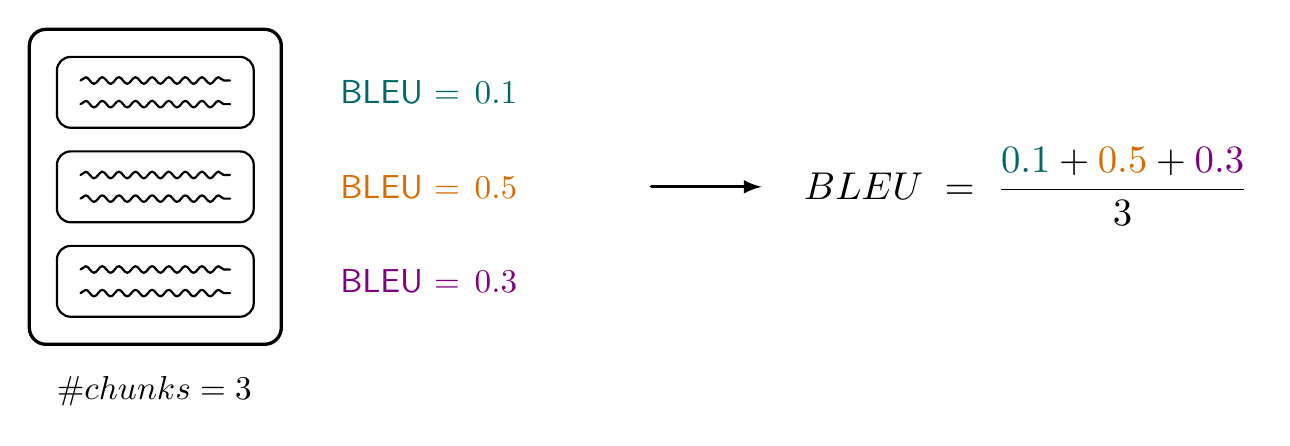
\begin{tikzpicture}[line join=round,line cap=round, >=latex, font=\sffamily]

% --- Left black container with three chunks ---
\draw[black, very thick, rounded corners=6pt]
  (-0.2,3.6) rectangle (3.0,-0.4);

% three inner rounded rectangles
\foreach \y in {2.8,1.6,0.4}{
  \draw[black, thick, rounded corners=5pt] (0.15,\y+0.45) rectangle (2.65,\y-0.45);
  % squiggle inside
  \draw[black, thick, decorate, decoration={snake,amplitude=1.2pt,segment length=6pt}]
    (0.45,\y-0.15) -- (2.35,\y-0.15);
  \draw[black, thick, decorate, decoration={snake,amplitude=1.2pt,segment length=6pt}]
  (0.45,\y+0.15) -- (2.35,\y+0.15);
}

% --- Colored BLEU labels next to each chunk ---
\node[anchor=west, text=teal!80!black, scale=1.2]  at (3.6,2.8) {BLEU $=\,0.1$};
\node[anchor=west, text=orange!85!black, scale=1.2] at (3.6,1.6) {BLEU $=\,0.5$};
\node[anchor=west, text=violet, scale=1.2]         at (3.6,0.4) {BLEU $=\,0.3$};

% --- n_chunks = 3 (black) ---
\node[anchor=west, text=black, scale=1.2] at (0.0,-1.0) {$\#\text{ chunks}=3$};

% --- Arrow to the right and mean BLEU expression ---
\draw[black, very thick, ->, >=latex] (7.7,1.6) -- (9.1,1.6);

\node[anchor=west, text=black, scale=1.4] at (9.3,1.6)
  {$\varnothing\ \text{BLEU} \;=\; \displaystyle
   \frac{\textcolor{teal!80!black}{0.1}+\textcolor{orange!85!black}{0.5}+\textcolor{violet}{0.3}}{3}$};

\end{tikzpicture}
}
  \caption[Computation of the mean \ac{bleu} score over chunks.]{Computation of the mean \ac{bleu} score over three text chunks of a text.}
  \label{fig:mean-bleu}
\end{figure}


\subsection{Exp.\ 4: Comparing Prompts}
\label{subsec:prompt_impact_setup}

Since the \impAppr{} relies on paraphrased texts as a basis for further computation, it is crucial to ensure that these paraphrases are both on topic and of comparable length as their reference.  
Large variations in length may introduce confounding effects, diminishing the reliability of subsequent analyses.
This experiment aimed to investigate how different prompting strategies affect the quality of paraphrases generated by \acp{llm}. 
Specifically, it was designed to address two key questions:
\begin{enumerate}
\item How strongly does the choice of prompt influence the length of generated paraphrases $p$ relative to their reference text $r$ across different \acp{llm}?
\item Which prompt most effectively mitigates the confounding effect of paraphrase length?
\end{enumerate}

We designed three prompt variants (cf. \Cref{subsec:one_step_paraphrasing_prompts}) to instruct models in the paraphrasing task.
The first prompt, i.e.\ \texttt{prompt0}, directs the model to paraphrase by substituting the main subject, verb, and object with synonyms, keeping the output close in length to the reference.  
The second prompt, i.e.\ \texttt{prompt1}, requests a paraphrase that varies wording and sentence structure while preserving tone, with length similar to the original.  
The third prompt, i.e.\ \texttt{prompt2}, instructs the model to produce a paraphrase three times longer than the reference, while preserving meaning and tone. 

We selected reference texts from our datasets and applied the prompts to four autoregressive \acp{llm}, choosing causal models because their architecture better supports text generation than masked models. 
The models include \texttt{meta-llama-3.1-8b-instruct}, \texttt{mistral-large-instruct}, \texttt{qwen3-32b}, and \texttt{openai-gpt-oss-120b}.
Further architectural details are provided in \Cref{app:language_models} of the Appendix. 

We generated paraphrases for each model–prompt pair.
The evaluation focused on two main aspects. 
Since length acts as a confounding variable for \imps{}, we measured the relative length difference $d = \frac{\mathrm{len}(p)}{\mathrm{len}(r)}\times 100 \%$ between each reference text $t$ and its paraphrase $r$. 
Additionally, we manually inspected long paraphrases and those of similar length to their references to verify semantic preservation and readability.


% \subsection{Exp.\ 4: Impact of Syntactic Similarity on \impApprTitle{} Performance}
\label{sec:syn_sim_impact_}

We designed this experiment in order to assess whether the syntactic similarity of generated paraphrases, i.e.\ the difficulty of hard negatives, influences the effectiveness of the \impAppr{}.
We conducted this experiment on both the \dataBlog{} and \dataStudent{} datasets, selecting 15 samples each from the training and test splits. 
The detector was configured according to Table~\ref{tab:imp_syn_sim_config}.

\begin{table}[h]
\centering\small
\caption{Exp.\ 4: \impAppr{} configuration.}
\label{tab:imp_syn_sim_config}
\begin{tabular}{@{}rlrrl@{}}   % numbers should be right aligned, text left aligned
\toprule
\# Impostors & Generation & Rounds & Top $n$ & Upsample \\
\midrule
50 & LLM & 100 & \num{100000} & False \\
\bottomrule
\end{tabular}%
\end{table}

For generation, we loop through all \ac{llm}-based paraphrasers until we successfully created 50 \imps{}.
One-step paraphrasers are used with both prompts.
Predictions on the test set were obtained by thresholding the detector’s scores with a decision threshold was determined using Youden’s J statistic on the training set.
We computed the average syntactic similarity on the test set. 
Following \citet{gohsen_captions_2023}, we define average syntactic similarity $\diameter_{syn}$ as the mean of the \ac{bleu}, \ac{rouge}-1, and \ac{rouge}-L scores. 
For each input pair in the test set, we calculated
(1) the average syntactic similarity between the two texts in the pair, (2) the mean average syntactic similarity between the candidate reference text and its paraphrases, and (3) the mean average syntactic similarity between the disputed text and the paraphrases.

We further grouped samples based on (1), (2), (3) and the difference (2)–(1). 
For each group, we computed accuracy, precision, recall, and F1 score of the detector’s predictions. 
The average values for each metric in a bin are presented in a bar chart.



% \subsection{Exp. 5: Comparing \acs{av} Methods in Traditional Human-Human Scenario}
\label{subsec:imp_gen}

We want to answer the question of how our \ac{llm}-based \imp{} generation performs compared to (a) traditional \imp{} generation methods in the \impAppr{}~\citep{koppel_determining_2014}, and compared to (b) \acl{sota} \ac{av} methods in the traditional \ac{av} scenario.
We thus, create 10 same- and 10 different-author pairs from the \dataStudent{}. % (llm_detection_scenarios.py)
% We thus, create 100 same- and 100 different-author pairs from the \dataStudent{} (comp_av.py)
% 1 each on and the \dataBlog{} datasets % 1 for Blog, 100 for Student Essays
It is noteworthy, that an approach predicting only one output will obtain an accuracy of $0.5$.
The \impAppr{} and \unmasking{} detector configuration are shown in \autoref{tab:exp5_imp_config} and \autoref{tab:exp5_unmasking_config}, respectively.

\begin{table}[h]
\centering\small
\caption{Exp. 5: \impAppr{} configurations.}
\label{tab:exp5_imp_config}
\begin{tabular}{@{}rlrrl@{}}   % numbers should be right aligned, text left aligned
\toprule
\# Impostors & Generation & Rounds & Top $n$ & Upsample \\
\midrule
50 & \textit{Variable} & 100 & \num{100000} & False \\
\bottomrule
\end{tabular}%
\end{table}

\begin{table}[h]
\centering\small
\caption[Exp. 5: Unmasking configurations.]{Exp. 5: Unmasking configurations. CV denotes cross-validation.}
\label{tab:exp5_unmasking_config}
\begin{tabular}{@{}rrrrl@{}}   % numbers should be right aligned, text left aligned
\toprule
\# CV Folds & \# Chunks & Rounds & Top $n$ & Upsample \\
\midrule
3 & 60 & 30 & \num{250} & False \\
\bottomrule
\end{tabular}%
\end{table}

For each impostor generation method, we computed accuracy, precision, recall, and F1 score for different thresholds. 


% \subsection{Comparing \ac{av} Methods}

This experiment evaluates the performance of the \impAppr{} in comparison to established \ac{av} methods.
As baselines, we employ generalized unmasking~\citep{bevendorff_generalizing_2019} and the compression-based approach PPMD approach.
All methods share the common characteristic of operating on lower-dimensional representations of the input text pair to determine whether both texts originate from the same author.

Following the experimental setup described in \autoref{subsec:imp_gen}, we assess performance using  accuracy, precision, recall, and the F1 score. 





